\Chapter{Neurális hálók}

A neurális hálózattokat \cite{neuralis77} gyakran hasonlítjuk az emberi agy működéséhez. Ha körültekintően szemügyre vesszük agyunk működését, akkor azt tapasztaljuk, hogy neuronokból és közöttük felépülő kapcsolatokból áll össze. A külvilágból érkezett ingereket értelmezhetjük úgy, mint egy bemenetet, amit az agyunkban lévő neuronok feldolgoznak.

A neurális hálózatokat gyakran hasonlítjuk az emberi agy működéséhez. Ha körültekintően szemügyre vesszük agyunk működését, akkor azt tapasztaljuk, hogy neuronokból és közöttük felépülő kapcsolatokból áll össze. A külvilágból érkezett ingereket értelmezhetjük úgy, mint egy bemenetet, amit az agyunkban lévő neuronok feldolgoznak.

\begin{figure}[h]
	\centering
	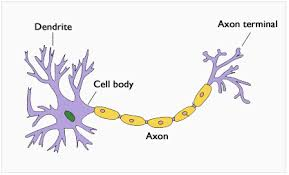
\includegraphics[scale=1.0]{images/neuron.png}
	\caption{A biológiai neuron fő részei}
	\label{fig:neuron}
	(forrás: \url{https://blog.vivekpanyam.com/deep-learning-made-simple-part-1/})
\end{figure}

A kutatók az agy felépítését vizsgálva egy olyan matematikai modellt dolgoztak ki, amely   reprezentálni próbálja az agyban található neuronokat  és a közöttük lévő kapcsolatokat. (Az agyban lévő neuron sematikus felépítését láthatjuk \aref{fig:neuron}. ábrán.) Ezt a modellt nevezzük neurális hálónak vagy neurális hálózatnak.

A neurális hálózatot alkotó neuronok úgynevezett rétegekbe rendeződnek. Háromféle réteget különbözetünk meg, a \textbf{\textit{bemeneti}}, a \textbf{\textit{kimeneti}} és a \textbf{\textit{rejtett réteget}}. Bemeneti és kimeneti rétegből minden hálózatban egy darab van, rejtett rétegből azonban tetszőleges számú lehet.

A hálózatban a rétegeket élek kötik össze egymással, amelyekhez egyenként egy-egy \textbf{\textit{súly}} tartozik. A neuronok a bemeneti éleiken kapott értékek és a súlyok segítségével bizonyos műveleteket végeznek el, majd az eredmény a kimeneti éleiken keresztül továbbítják a következő réteg neuronjai felé.

A tanítási folyamat elvégzésekor a hálózatba olyan bemenetet juttatunk, amelyhez tartozó kimenet ismert. A bemenetet végig futtatjuk a hálózat rétegein, majd a kimeneti réteg által szolgáltatott eredményt összehasonlítjuk a kimenet várt értékével. A két érték közötti eltérést a hálózat \textit{\textbf{hibájának}} nevezzük. A tanítás folyamán a hálózat súlyait úgy változtatjuk, hogy ez a hiba lehetőleg minél kisebb legyen. A hálózat betanítása után már olyan bemeneteket is megadhatunk, amelyeknek nem ismerjük a kimenetét, és a hálózat ezekre is képes hibahatáron belüli kimenetet produkálni.

\begin{figure}[h]
	\centering
	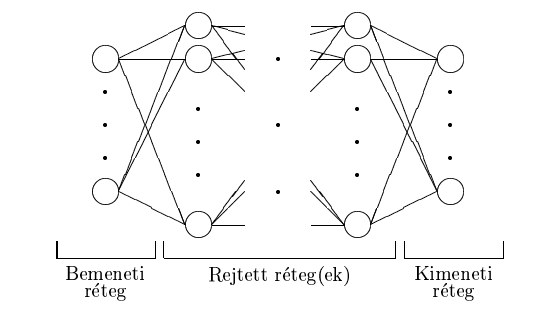
\includegraphics[scale=0.75]{images/ANNLayers.png}
	\caption{Egy általános felépítésű neurális hálózat (forrás: \cite{neuralis77})}
\end{figure}

\section{A neurális hálók elemei}

Az egyszerűség kedvéért vizsgáljunk meg egy olyan neurális hálózatot, amelynek egyetlen neuronnal rendelkezik. Ezt szokás \textbf{\textit{Perceptron}}-nak is nevezni.

\textbf{\textit{Bemenet}}: Az kiértékelendő adat (ember számára ingerek), amit általában egy vektor (jelölje $x$) reprezentál.

\textit{\textbf{Súlyok}}: Két neuron közötti kapcsolat. Egy valós érték. A hálózat súlyait mátrixba tároljuk el (ezt jelölje $W$).

\textbf{\textit{Összegző csomópont}}: A bemeneteket összeszorozza a megfelelő súlyokkal és ezek összegét képezi. Tulajdonképpen mátrix szorzásról van szó.

$$
v(n) = \sum_{i=1}^{n}(w_ix_i)
$$

\textit{\textbf{Aktivációs függvény}}: Egy olyan függvény ($\varphi$), ami leképezi a kapott összeget egy adott intervallumba, amely általában a $[0, 1]$ vagy $[-1, 1]$ intervallumokat jelenti.

\textbf{\textit{Kimenet}}: A leképezett értékünk lesz a kimenetünk (jelölje $y$).

\begin{figure}[h]
	\centering
	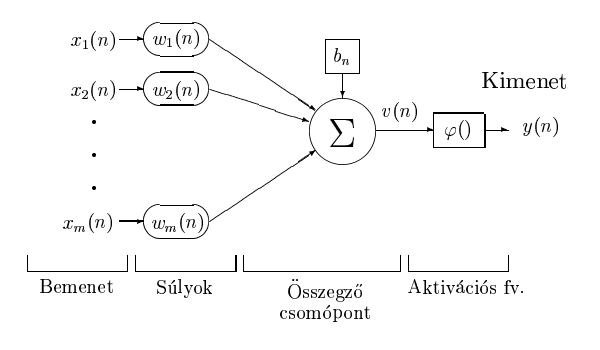
\includegraphics[scale=0.6]{images/ANNParts.png}
	\caption{A matematikai neuron modell felépítése (forrás: \cite{neuralis77})}
	\label{fig:ANNParts}
\end{figure}

\Aref{fig:ANNParts}. ábrán láthatjuk a mesterséges neurális háló neuronjának matematikai modelljét. Ebben a $b_n$ változót \textit{bias}-nak nevezzük. A bias érték általában egy olyan bemenet, amely akkor is lehetővé teszi az $1$-es kimeneti értéket, ha a bemeneten $0$ érték szerepel. Ez kritikus fontoss-gú lehet a sikeres tanuláshoz. Tegyük fel hogy a neurális hálózat egy függvény: $y = mx$. A fenti függvény az origót metszi, ami nem minden esetben add jó eredményeket. A bias definiálásával a függvényünk kap egy konstans paramétert $y = mx + b$. A $b_n$-hez tartozó súly ($w_b$) általában -1 vagy 1.

Amennyiben az $x(n)$ bemenethez tartozó ideális kimenetet $d(n)$-nel jelöljük, illetve $y(n)$ jelenti a hálózat által az $x(n)$ bemenetre adott kimenetét, a neurális hálózat négyzetes hibáját a következőképpen értelmezzük:
$$
\varepsilon = (d(n) - y(n))^2.
$$

Ezt a hibát akarjuk a tanítási eljárás során minimálisra csökkenteni. Természetesen az lenne az ideális, ha a hibát egészen nullára tudnánk redukálni, de ez általában nem sikerül, ezért meg kell elégednünk egy kellően kicsiny hibaküszöbbel.

Aktivációs függvényként tetszőleges balról illetve jobbról folytonos eloszlásfüggvény megfelel, azaz olyan függvényt kell választanunk, amely
\begin{itemize}
\item monoton növekvő,
\item balról/jobbról folytonos,
\item határértéke $+\infty$-ben 1, $-\infty$ -ben 0.
\end{itemize}

Aktivációs függvénynek általában a szigmoid, azaz S alakú, függvényeket használjuk (mint például a logisztikus, tangens hiperbolikus függvények).

Az aktivációs függvényeknél egy úgynevezett rámpafüggvényről (RELU), ami az
$$
f(x) = max(0,x)
$$
összefüggéssel írható le, ahol $x$ az aktivációs függvény bemenete (\ref{fig:relu}. ábra).

\begin{figure}[h]
\centering
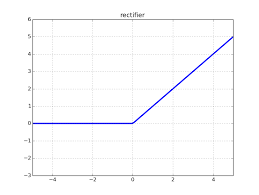
\includegraphics[scale=1.0]{images/relu}
\caption{A rámpafüggvény}
\label{fig:relu}
(forrás: \url{https://sefiks.com/2017/08/21/relu-as-neural-networks-activation-function/})
\end{figure}

A legújabb biológiai kutatások és a gyakorlati tapasztalatok is igazolják hogy a RELU-val történő tanítások szignifikánsan jobban teljesítenek. Legnagyobb előnye a regressziós tanítások esetén mutatkozik meg.

\section{A Backpropagation tanítási algoritmus}

Hiba minimalizálása során szükségünk van az aktuális hibára. Az összes kimeneti neuronra kiszámoljuk a négyzetes hibát és ezeket összeadjuk:
$$
E_{total} = \sum \dfrac{1}{2}(target - output)^2.
$$
(Az $\dfrac{1}{2}$ szorzót azért használjuk hogy el tudjuk távolítani majd a kitevőt a későbbiekben deriváláskor.)

A backpropagation célja, hogy frissítse az egyes súlyokat a hálózaton úgy, hogy az aktuális kimenet közelebb kerüljön a célkimenethez, ezáltal minimalizálva az egyes kimeneti neuronok és a hálózat egészének hibáját. A backpropagation algoritmus számításaira láthatunk egy példát \aref{fig:ANN_backprog}. ábrán.

\begin{figure}[h]
\centering
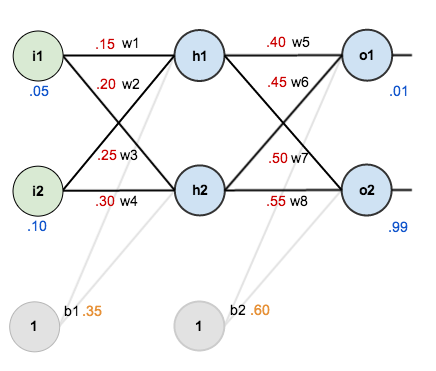
\includegraphics[scale=0.5]{images/ANN_backprog}
\caption{Példa a visszaterjesztéses tanítás alkalmazására}
(forrás: \url{https://mattmazur.com/2015/03/17/a-step-by-step-backpropagation-example/})
\label{fig:ANN_backprog}
\end{figure}

Tekintsük a $w_5$-öt. Azt szeretnénk tudni, hogy a $w_5$ változása milyen hatást gyakorol a teljes hibára, más néven $\frac{\partial E_ {total}}{\partial w_ {5}}$. Úgy is fogalmazhatunk hogy a gradiens a $w_5$ vonatkoztatásba.

Ezt a láncszabály alkalmazásával tudjuk kiszámolni:
$$
\frac{\partial E_{total}}{\partial w_{5}} = \frac{\partial E_{total}}{\partial out_{o1}} \cdot \frac{\partial out_{o1}}{\partial net_{o1}} \cdot \frac{\partial net_{o1}}{\partial w_{5}}.
$$

Lássuk az egyenlet elemeit!
\begin{flushleft}
\begin{equation}
E_{total} = \frac{1}{2}(target_{o1} - out_{o1})^{2} + \frac{1}{2}(target_{o2} - out_{o2})^{2}
\end{equation}
\begin{equation}
\frac{\partial E_{total}}{\partial out_{o1}} = 2 \cdot \frac{1}{2}(target_{o1} - out_{o1})^{2 - 1} \cdot (-1) + 0
\end{equation}
\begin{equation}
\frac{\partial E_{total}}{\partial out_{o1}} = -(target_{o1} - out_{o1}) = -(0.01 - 0.75136507) = 0.74136507
\end{equation}

\end{flushleft}

A logisztikus függvény parciális deriváltja a kimenet szorzata (1 - kimenet):
$$
out_{o1} = \frac{1}{1+e^{-net_{o1}}}
$$

$$
\frac{\partial out_{o1}}{\partial net_{o1}} = out_{o1}(1 - out_{o1}) = 0.75136507(1 - 0.75136507) = 0.186815602
$$

Végül, mennyire változik az $o1$ változó teljes bemenete a $w_5$ tekintetében?
$$
net_{o1} = w_5 \cdot out_{h1} + w_6 \cdot out_{h2} + b_2 \cdot 1
$$

$$
\frac{\partial net_{o1}}{\partial w_{5}} = 1 \cdot out_{h1} \cdot w_5^{(1 - 1)} + 0 + 0 = out_{h1} = 0.593269992
$$

Összesítve az eddigieket:
$$
\frac{\partial E_{total}}{\partial w_{5}} = \frac{\partial E_{total}}{\partial out_{o1}} \cdot \frac{\partial out_{o1}}{\partial net_{o1}} \cdot \frac{\partial net_{o1}}{\partial w_{5}}
$$

$$
\frac{\partial E_{total}}{\partial w_{5}} = 0.74136507 \cdot 0.186815602 \cdot 0.593269992 = 0.082167041
$$

A hiba csökkentése érdekében kivonjuk ezt az értéket az aktuális súlyból (adott esetben szorozva egy bizonyos tanulási sebességgel, $\eta$, amelyet 0,5-re állítunk):
$$
w_5^{+} = w_5 - \eta \cdot \frac{\partial E_{total}}{\partial w_{5}} = 0.4 - 0.5 \cdot 0.082167041 = 0.35891648
$$

Meg tudjuk ismételni ezt a folyamatot, hogy megkapjuk az új súlyokat $w_6$, $w_7$ és $w_8$:
$$
w_6 ^ {+} = 0,408666186
$$

$$
w_7 ^ {+} = 0.511301270
$$

$$
w_8 ^ {+} = 0.561370121
$$

Ezután folytatjuk a hátrafelé az új értékeket a $w_1$, $w_2$, $w_3$ és $w_4$ értékek kiszámításával. Hasonlóan láncszabályt alkalmazunk. A visszaterjesztés módjának egy szemléltetését \aref{fig:ANN_bp_viz}. ábrán láthatjuk.

\begin{figure}[h]
\centering
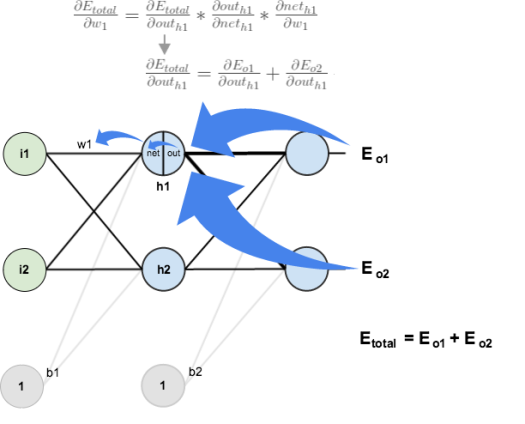
\includegraphics[scale=0.5]{images/ANN_bp_viz}
\caption{A hiba visszaterjesztése a súlyok módosításához}
\label{fig:ANN_bp_viz}
(forrás: \url{https://mattmazur.com/2015/03/17/a-step-by-step-backpropagation-example/})
\end{figure}

Végül frissítjük az összes súlyunkat. Amikor eredetileg a 0.05 és a 0.1 bemeneteket továbbítottuk, a hálózat hibája 0.2983711 volt. A backpropagation első fordulója után a teljes hiba 0.2910279 értékre csökken. Lehet, hogy nem tűnik soknak, de miután megismételtük ezt a folyamatot 10 000-szer, a hiba lecsökken 0.0000351-re.

\section{Konvolúciós neurális hálózat}

A konvolúciós neurális hálózat hagyományos neurális hálózat alapokon nyugszik \cite{liconvolution}. Annak egy speciális fajtája, amit képeken található minták feltárására fejlesztettek. Neuronokból épülnek fel és hasonlóképpen rendelkeznek tanítható súlyokkal. A bemeneteiken kapott értékek skaláris szorzatát egy nem lineáris leképezés követheti. Az egész hálózat reprezentálhat egy egyszerű osztályozó eljárást, aminek a bemenetei a nyers képpontok, és a kimenete lehet egy adott kép osztályba tartozás valószínűsége. A mi esetünkbe a bemenet a kínai karakter pixel értékei, a kimenet pedig valószíűségek a karakterekből adódóan.

A konvolúciós neurális hálózat hagyományos neurális hálózat alapokon nyugszik. Annak egy speciális fajtája, amit eredendően képeken található minták feltárására fejlesztettek. Neuronokból épülnek fel és hasonlóképpen rendelkeznek tanítható súlyokkal. A bemeneteiken kapott értékek skaláris szorzatát egy nem lineáris leképezés követheti. Az egész hálózat reprezentálhat egy egyszerű osztályozó eljárást, aminek a bemenetei a nyers képpontok, és a kimenete lehet egy adott kép osztályba tartozás valószínűsége. A mi esetünkben a bemenet a kínai karakterek pixel értékei, a kimenet pedig egy becsült osztályba tartozási mérték.

A hagyományos neurális hálózatok nem skálázzák a teljes képet. A kínai (különösen a hagyományos) több száz karaktert nem lehet megjeleníteni egy $16 \times 16$ pixeles rácsban. A megfelelő méret körülbelül $24 \times 24$ képpontot tartalmaz. Neurononként $24 \times 24 = 526$ súly paramétert jelentene. Ez még kezelhetőnek tűnik, de tisztán látszik, hogy a teljesen összekapcsolt struktúra nem kezeli jól a képeket.

Ha végig gondoljuk, hogy az hány paramétert jelent még egy kis neuronszámú kevés rejtett rétegből álló hálózat esetében, akkor rájöhetünk, hogy nagyobb méretű képen fellelhető minták felismeréséhez a hagyományos neurális hálózatok alkalmazása nem célravezető, emiatt a kép előfeldolgozására, szűrésére konvolúciós rétegeket vezetnek be.

\subsection{A háló felépítése}

A konvolúciós neurális hálózatokban szereplő rétegeket funkció alapján alapvetően két csoportra lehet bontani.

\begin{enumerate}
\item A konvolúciós rétegek, amik - mint paraméterezhető szűrők - előfeldolgozást végeznek a képen. Ezáltal a kép mérete lecsökken, a hordozott információtartalom kiemeltté válik.
\item A hagyományos neurális hálózat (második csoport) számára feldolgozható lesz, az osztályozást el tudja végezni. Egy konvolúciós neurális hálózat tehát konvolúciós és hagyományos rejtett rétegekből épül fel.
\end{enumerate}

A konvolúciós rétegek alapjában véve színes képek feldolgozására lettek kifejlesztve, ezért a neuronjaik három dimenzióban (szélesség, magasság, színcsatornák) vannak elrendezve.

A mi esetünkbe fekete-fehér képek állnak rendelkezésre. A színes képek esetén grayscale konvertálást végezhetünk el. Ha a pixel érték fekete akkor 0-át, ha fehér akkor 255-et rendelünk hozzá. A szürke árnyalatokat $[0, 255]$ közötti értékekkel definiáljuk. Egy kínai karakterre \aref{fig:chinese_char_pixel}. ábrán láthatunk példát.

\begin{figure}[h]
\centering
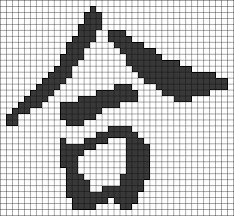
\includegraphics[scale=0.65]{images/chinese_char_pixel}
\caption{Egy kínai karakter fekete-fehér raszteres képként}
\label{fig:chinese_char_pixel}
\end{figure}

A következő felsorolásban - a tipikus, de nem kizárólagos sorrendre ügyelve - bemutatnám a konvolúciós hálózat rétegtípusait:

\begin{itemize}
\item \textit{Bemeneti réteg}: Tartalmazza a kép nyers pixel értékeit. Az értékeket sorba állítjuk és azokat egy 1 dimenziós vektor reprezentálja, ami 0 és 1 értékeket tartalmaz.

\item \textit{Konvolúciós réteg}: Adott képpont csoportokra konvolúció matematikai műveletet alkalmazunk. A konvolúció eredménye egy skalár (a skaláris szorzata a kép egy adott részének és a szűrőnek). Ha minden képpont csoportra elvégezzük a konvolúciót, akkor egy aktivációs térképet kapunk. Általában több szűrő paraméterrel is elvégezzük a konvolúciót és aktivációs térképeket egymásra rakjuk. Az aktivációs térkép, a művelet tulajdonsága miatt, kisebb
méretű lesz (\ref{fig:convolution}. ábra).

\begin{figure}[h]
\centering
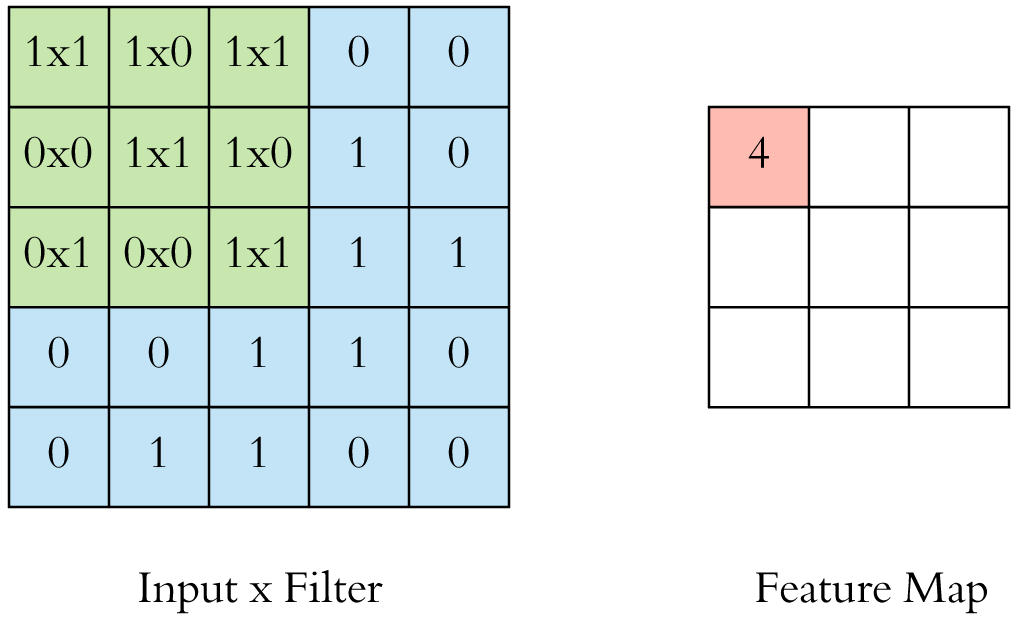
\includegraphics[scale=0.3]{images/convolution}
\caption{A bináris mátrix és a belőle konvolúcióval kinyert jellemzők}
(forrás: \url{https://towardsdatascience.com/applied-deep-learning-part-4-convolutional-neural-networks-584bc134c1e2})
\label{fig:convolution}
\end{figure}

Konkrétan mátrix szorzásról van szó. A feature map elemei egész számok, amik további konvolúciós rétegen mennek keresztül. Lehet közben különböző szűröket is használni.

A \textit{keras} nevű Python csomagban ennek megvalósítása az alábbi módon lehetséges.
\begin{python}
from keras.models import Sequential
from keras.layers import Dense, Dropout, Flatten
from keras.layers import Conv2D, MaxPooling2D

model = Sequential()
model.add(Conv2D(64, (3, 3),
	weights=[np.random.normal(0, 0.01,
	size=(3, 3, 1, 64)), np.zeros(64)],
	activation='relu', padding='same',
	strides=(1, 1),
	input_shape=(1, 64, 64)))
\end{python}

\item \textit{RELU réteg}: A konvolúciós réteg aktivációs függvénye, ami a következő leképezést valósítja meg: $f(x) = max(x, 0)$. Vagyis, ha a bemenet kisebb, mint nulla, akkor a kimenet nulla lesz, ha nagyobb, mint nulla, akkor a kimenet a bemenet értékét veszi fel. A konvolúciós hálóknál a RELU sokkal gyorsabb más aktivációs függvényeknél, mint például a sigmoid vagy a tanh.
\item \textit{Összevonó réteg (pooling layer)}: A Pooling Layer függetlenül működik minden egyes feature map-nél. A MAX művelet segítségével kinyeri a legfontosabb vonásokat, csökkentve a dimenzióját. A leggyakoribb forma egy $2 \times 2$-es méretű szűrő, melyet 2 lépéssel kell felvinni minden szeletre. A bemenetben 2 szélesség és magasság mellett, az aktiválások 75\% -át eldobja. Minden MAX művelet ebben az esetben 4 számot vesz igénybe. Ennek használatát az alábbi kódpélda mutatja.
\begin{python}
model.add(MaxPooling2D(pool_size=(2, 2), strides=(2, 2)))
\end{python}

\begin{figure}[h]
\centering
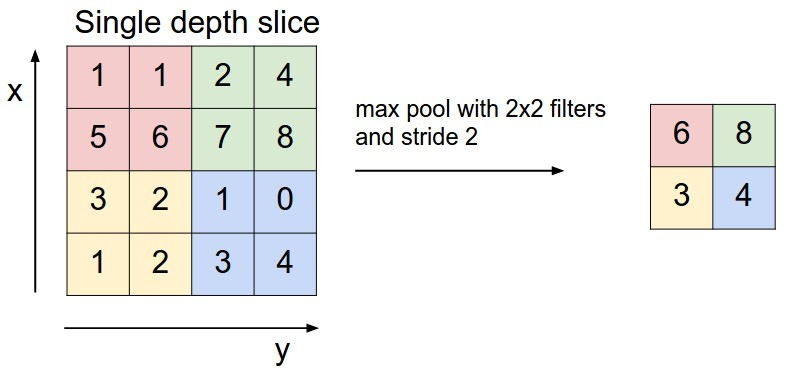
\includegraphics[scale=0.3]{images/maxpool}
\caption{A pooling réteg működése egy példán keresztül}
\label{fig:maxpool}
(forrás: \url{http://cs231n.github.io/convolutional-networks/})
\end{figure}

\item \textit{Teljesen összekötött réteg (fully connected, FC)}: Utolsó rétegekként szokták használni, hagyományos réteg. Lehet 1 vagy több réteg is a feladattól függően. Az osztályozás rész itt történik. A kimenetek valószínűségek a felsorolt karakterek szerint.
\begin{python}
model.add(Dense(200, activation='softmax'))
\end{python}
\end{itemize}

\Aref{fig:CNN_CCR_working}. ábra egy konvolúciós feldolgozást mutat be, ahol szemléltetve vannak az egyes rétegek utáni állapotok. A képen látható az egyes konvolúció utáni állapotok tulajdonság érzékelőként viselkednek.

\begin{figure}[h]
\centering
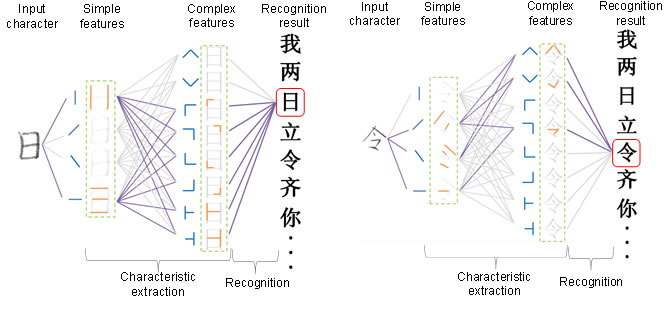
\includegraphics[scale=0.65]{images/CNN_CCR_working}
\caption{A konvolúciós karakterfelismerő hálózat sematikus felépítése}
(forrás: \url{http://www.fujitsu.com/global/Images/20130821-01b_tcm100-929717.jpg})
\label{fig:CNN_CCR_working}
\end{figure}

\subsection{Hálózat architektúra}

A megfelelő háló architektúra megválasztása nagyon fontos a tervezési szakasznál. A következőkben egy 2013-as eredményt mutatok be, miszerint a rétegek és a bennük lévő neuronok számával csökkenthető a hibaarány \cite{cirecsan2015multi}.

Először vessünk egy pillantást az adathalmazunkra. Az adat egyszerű képeket tartalmaz (offline kép). Tartalmaz 224419 karaktert, amelyeket 60 személy írt. A karakterek $48 \times 48$ pixelre skálázták. Az előfeldolgozás OpenCV-vel történik.

Nyolc hálózaton történt tanítás. Minden hálózatnak 11 rétege van, beleértve a bemeneti és kimeneti réteget. A jellemzők kinyerés fázisánál 100-450 darabszámú neuront használ. Végezetül két egymást követő teljesen összekötött (fully-connected) hálózat végzi el az osztályozást.

Tehát $48 \times 48$ bemeneti réteg, $xCy$ konvolúciós réteg, ahol $x$ neuronok (maps) száma és $y$ a szűrő mérete ($y \cdot y$). Az $MPy$ az összevonó réteg (max-pooling), ahol az $y$ a pooling méret ($y \cdot y$). Az $xN$ pedig a teljesen összekötött hálózat, ahol az $x$ a neuronok számát jelöli.

\begin{table}[h]
\centering
\begin{tabular}{|l|l|l|}
\hline
 Háló &                                                                      & Hiba[\%] \\ \hline
0               & 48x48-150C3-MP2-250C2-MP2-350C2-MP2-450C2-MP2-1000N-3755N & 5.528 \\ \hline
1               & 48x48-150C3-MP2-250C2-MP2-350C2-MP2-450C2-MP2-1000N-3755N & 5.931 \\ \hline
2               & 48x48-300C3-MP2-300C2-MP2-300C2-MP2-300C2-MP2-1000N-3755N & 5.792 \\ \hline
3               & 48x48-100C3-MP2-200C2-MP2-300C2-MP2-400C2-MP2-500N-3755N  & 5.625 \\ \hline
4               & 48x48-100C3-MP2-200C2-MP2-300C2-MP2-400C2-MP2-1000N-3755N & 5.951 \\ \hline
5               & 48x48-100C3-MP2-200C2-MP2-300C2-MP2-400C2-MP2-1000N-3755N & 6.114 \\ \hline
6               & 48x48-100C3-MP2-200C2-MP2-300C2-MP2-400C2-MP2-1000N-3755N & 6.339 \\ \hline
7               & 48x48-100C3-MP2-200C2-MP2-300C2-MP2-400C2-MP2-500N-3755N  & 5.995 \\ \hline
\end{tabular}
\caption{Az egyes hálók hibaarányai (forrás:\url{https://arxiv.org/pdf/1309.0261.pdf})}
\label{tab:ann_result}
\end{table}

Észrevehető, hogy a rétegekben a neuronok növelése csökkenti a hibaarányt. Bizonyítható, hogy a pontosság és a robusztusság növekszik, ha neuronok száma nő (\ref{tab:ann_result}. táblázat).

A bonyolult hálózatok gyakran hajlamosak a túltanulásra, overfitting-re. Az overfitting azt jelenti, hogy a hálózat túl jól illeszkedik a tanitó mintára, ezért az nem fog jól teljesíteni a teszt mintára.

Ilyenkor lehet kezdeményezni Dropout-ot, ami annyit jelent, hogy véletlenszerűen deaktiválunk neuronokat, annak érdekében, hogy a hálózat más útvonalakon haladva máshogy tanuljon. Ez Python-ban az alábbi kóddal valósítható meg.
\begin{python}
model.add(Dropout(0.5))
\end{python}

\begin{figure}[h]
\centering
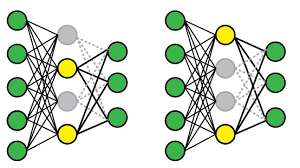
\includegraphics[scale=0.8]{images/dropout}
\caption{Neuronok véletlenszerű deaktiválása}
\label{fig:dropout}
\end{figure} 

\subsection{A háló tanítása}

Ez a neurális hálózatok használatának egyik lényeges pontja. Sok kérdés merülhet fel a megfelelő tanítási algoritmus kiválasztása közben.
\begin{itemize}
\item Hogyan ismerik az első konvolúciós rétegben lévő szűrők az élek és görbék keresését?
\item Hogyan ismeri fel a teljesen összekapcsolt réteg a jellemzőket?
\item Hogyan ismerik a szűrők az egyes rétegekben milyen értékeket kapnak?
\end{itemize}
A számítógép képes beállítani a szűrő értékeit (vagy súlyait) a backpropagation-nek nevezett eljárással.

A backpropagation négy különböző szakaszra osztható \cite{ABeginne32}:
\begin{itemize}
\item előre terjesztés (forward pass),
\item veszteség számítás (loss function),
\item hiba visszaterjesztés (backward pass),
\item súly frissítés (weight update).
\end{itemize}

Az előre terjesztés során egy kínai karakter képét (amelynek mérete például $48 \times 48$ pixel) továbbítunk az egész hálózaton. Az első leképzésnél, mivel minden súly és szűrőérték véletlenszerűen van inicializálva, így a kimenet is valószínűleg véletlenszerű lesz, ezért a hálózat nem add pontos osztályozást. A hálózat jelenlegi súlyaival nem tudja keresni az alacsony szintű jellemzőket, ilyenek például a stroke-ok. Emiatt tovább lépünk a veszteség számítás részre. Ne felejtsük el, hogy a tanító mintának van egy címkéje. A veszteségfüggvény többféle módon definiálható, de gyakori az \textit{MSE} (\textit{Mean Squared Error}, átlagos négyzetes hiba)
$$
E_{total} = \sum 1/2(target - output)^2.
$$ 

A \textit{target} egy vektor, aminek az értékei azt mutatják meg, hogy az adott minta a neurális háló döntése alapján mennyire illeszkedik a megfelelő karakterre. Ezt tipikusan úgy állítják össze, hogy a $0$ jelentse azt, hogy egyáltalán nem illeszkedik, az $1$ érték pedig, hogy a háló döntése alapján az a karakter teljesen illeszkedik.

A modell használatát mutatja az alábbi kódrészlet.
\begin{python}
model.compile(loss='categorical_crossentropy',
              optimizer='adadelta',
              metrics=['accuracy'])
\end{python}

A veszteség rendkívül magas az első képzésnél. Olyan pontra akarunk jutni, ahol az előre jelzett címke megegyezik a képzési címkével. Ahhoz, hogy odaérjünk, minimálisra csökkentjük a veszteségünket. Azt szeretnénk megtudni, hogy mely bemenetek/súlyok azok, amelyek leginkább hozzájárultak a hálózat veszteségéhez (vagy hibájához). Ezt az illeszkedést az alábbi módon határozhatjuk meg.

\begin{python}
model.fit(f['trn/x'], f['trn/y'],	
	validation_data=(f['vld/x'], f['vld/y']),
	epochs=15, batch_size=128,
	shuffle='batch', verbose=1)
\end{python}

A négyzetes hibafüggvény szemléltetését láthatjuk \aref{fig:CNN_loss}. ábrán.

\begin{figure}[h]
\centering
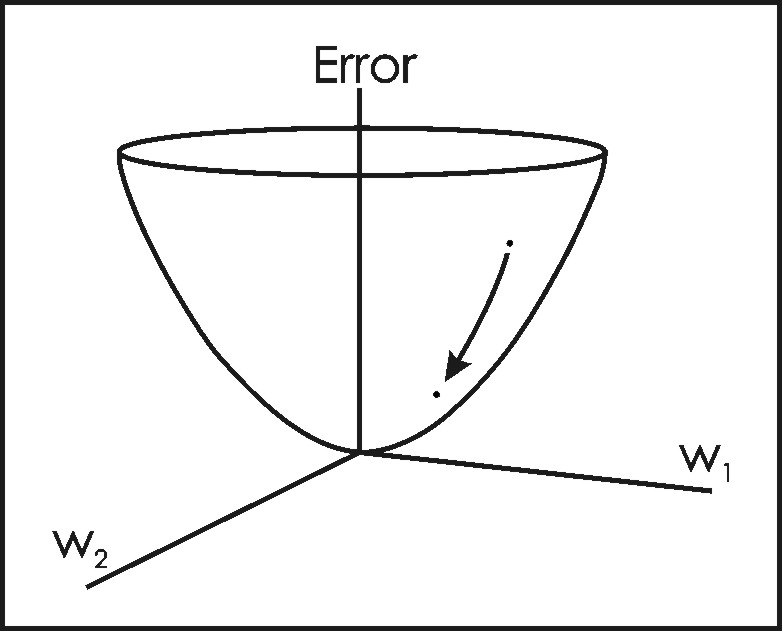
\includegraphics[scale=0.4]{images/CNN_loss}
\caption{A négyzetes hibafelület}
(forrás: \url{https://adeshpande3.github.io/A-Beginner%27s-Guide-To-Understanding-Convolutional-Neural-Networks/})
\label{fig:CNN_loss}
\end{figure}

A $dL/dW$ matematikai egyenlet írjuk fel a veszteség hozzájárulást. Következő lépés a hiba visszaterjesztés, amely meghatározza, hogy a súlyok milyen mértékben járultak hozzá a veszteséghez, és megtalálják azokat a módokat, amelyekkel a károk csökkenthetők. Miután kiszámítjuk ezt a származékot, akkor megyünk az utolsó lépéshez, amely a súlyok frissítése. Itt vesszük az összes súlyt és szűröt, és frissítjük őket úgy, hogy a gradiens ellenkező irányba változzon. Ekkor
$$
w = w_i - \eta \dfrac{dL}{dW},
$$
ahol $w$ a súly, a $w_i$ a kezdeti súly, az $\eta$ pedig a tanulási tényező.

A tanulási tényező egy olyan paraméter, amelyet a programozó választ. A magas tanulási arány azt jelenti, hogy nagyobb súlycsökkenést kell végrehajtani a súlycsökkentésekben, így kevesebb időre lehet szükség ahhoz, hogy a modell konvergáljon az optimális súlycsoporton. Azonban a túl magas tanulási arány olyan túl nagy ugrásokhoz vezethet, amelyek nem elég pontosak ahhoz, hogy elérjék az optimális pontot. Ennek egy szemléltetését láthatjuk \aref{fig:CNN_learning_rate}. ábrán.

\begin{figure}[h]
\centering
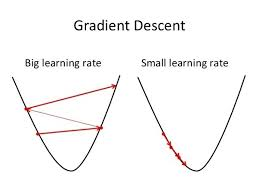
\includegraphics[scale=0.8]{images/CNN_learning_rate}
\caption{Magas és alacsony tanulási tényezők hatása}
(forrás: \url{https://adeshpande3.github.io/A-Beginner%27s-Guide-To-Understanding-Convolutional-Neural-Networks/})
\label{fig:CNN_learning_rate}
\end{figure}

Az előre terjesztés, a veszteség számítás, a visszaterjesztés és a paraméterfrissítés folyamata egy képzési iteráció. A program megismételi ezt a folyamatot egy rögzített számú iterációra. Miután befejezte a paraméter frissítést az utolsó képzésnél, remélhetőleg a hálózat megfelelően működik.

\subsection{Tesztelés}

Végül megnézzük, hogy működik-e a hálózat vagy sem. Különböző (még nem látott) képeket továbbíthatunk a CNN-en keresztül. Összehasonlítjuk a kimeneteket a címkékkel, és megnézzük a hibát. Ha alacsony hibát kapunk a hálózat jól dolgozott.

\subsection{Transfer learning}

A konvolúciós hálózatok betanításához nagyszámú mintára és nagy teljesítményű számítógépekre van szükség. Amennyiben nem áll rendelkezésünkre nagyjából egymillió képkockából álló tanító adathalmaz, akkor kis számú mintáról beszélünk. Ha nincs lehetőségünk vagy erőforrásunk nagy adathalmazzal tanítani, akkor is megvalósíthatjuk a kívánt leképezést. A transfer learning (tanulás átadása) módszer segítségével egy előre betanított hálózatot veszünk alapul, és annak utolsó pár rétegét lecserélve végezzük a tanítást. Ilyenkor a megmaradt rétegek betanított tulajdonság érzékelő funkciója segítségével a lecserélt rétegek által megvalósítandó leképezés könnyebbé vállhat. A konvolúciós neurális hálózatok tanítása esetében ez egy gyakori eljárás. Az interneten számos előre betanított hálózat található.
